\label{A5}
\subsection*{Introduction}

\D{} is designed to accommodate a number of different periodic boundary 
conditions\index{boundary conditions}, which are defined by the
shape and size of the simulation cell. Briefly, these are as follows
(which also indicates the IMCON flag defining the simulation cell type in
the CONFIG File - see \ref{configfile}):

\begin{enumerate}
\item None e.g. isolated polymer in space. (IMCON=0).
\item Cubic periodic boundaries\index{boundary conditions}.(IMCON=1).
\item Orthorhombic periodic boundaries.(IMCON=2).
\item Parallelepiped periodic boundaries.(IMCON=3).
\item Truncated octahedral periodic boundaries. (IMCON=4).
\item Rhombic dodecahedral periodic boundaries. (IMCON=5).
\item Slab (X,Y periodic, Z nonperiodic). (IMCON=6).
\item Hexagonal prism periodic boundaries. (IMCON=7).
\end{enumerate}

We shall now look at each of these in more detail. Note that in all
cases the cell vectors and the positions of the atoms in the cell are
to be specified in Angstroms (\AA).

\subsubsection*{No periodic boundary (IMCON=0)}

Simulations requiring no periodic boundaries are best suited to {\em
in vacuuo} simulations, such as the conformational study of an
isolated  polymer molecule. This boundary condition is not recommended
for studies in a solvent, since evaporation is likely to be a
problem. 

Note this boundary condition cannot be used with the Ewald summation
method.

\subsubsection*{Cubic periodic boundaries (IMCON=1)}

\begin{figure}[ht]
\begin{center}
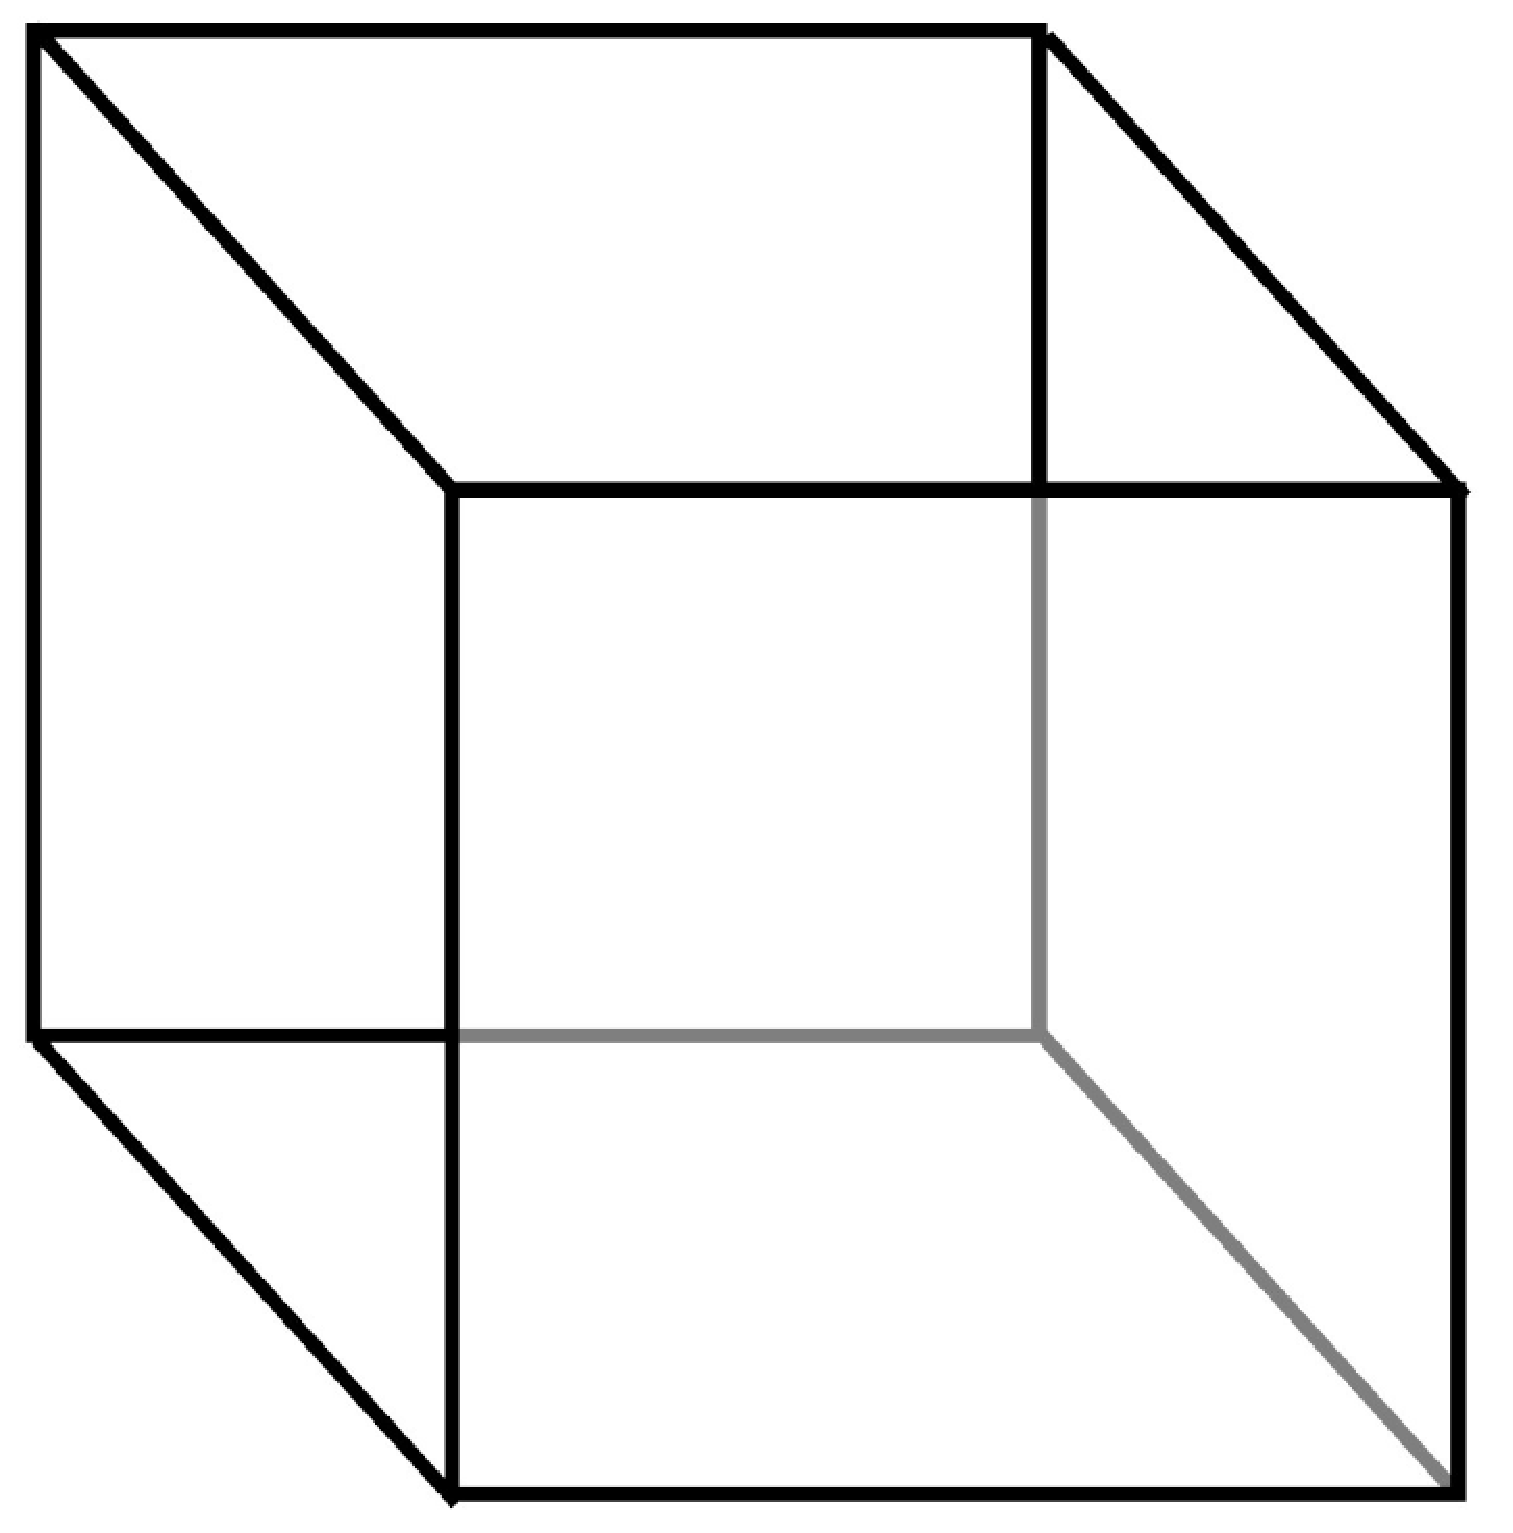
\includegraphics[height=5cm]{cube.ps}
\caption{The cubic MD cell.}
\end{center}
\end{figure}

The cubic MD cell is perhaps the most commonly used in simulation and
has the advantage of great simplicity. In \D{} the cell is defined with
the principle axes passing through the centres of the faces.  Thus for
a cube with sidelength D, the cell vectors appearing in the CONFIG
file should be: (D,0,0); (0,D,0); (0,0,D). Note the origin of the
atomic coordinates is the centre of the cell.

The cubic boundary condition can be used with the Ewald summation
method.

\subsubsection*{Orthorhombic periodic boundaries (IMCON=2)}
The orthorhombic cell is also a common periodic boundary, which
closely resembles the cubic cell in use. In \D{} the cell is defined
with principle axes passing through the centres of the faces.  For an
orthorhombic cell with sidelengths D (in X-direction), E (in
Y-direction) and F (in Z-direction), the cell vectors appearing in the
CONFIG file should be: (D,0,0); (0,E,0); (0,0,F). Note the origin of
the atomic coordinates is the centre of the cell.


The orthorhombic boundary condition can be used with the Ewald summation
method.

\begin{figure}[ht]
\begin{center}
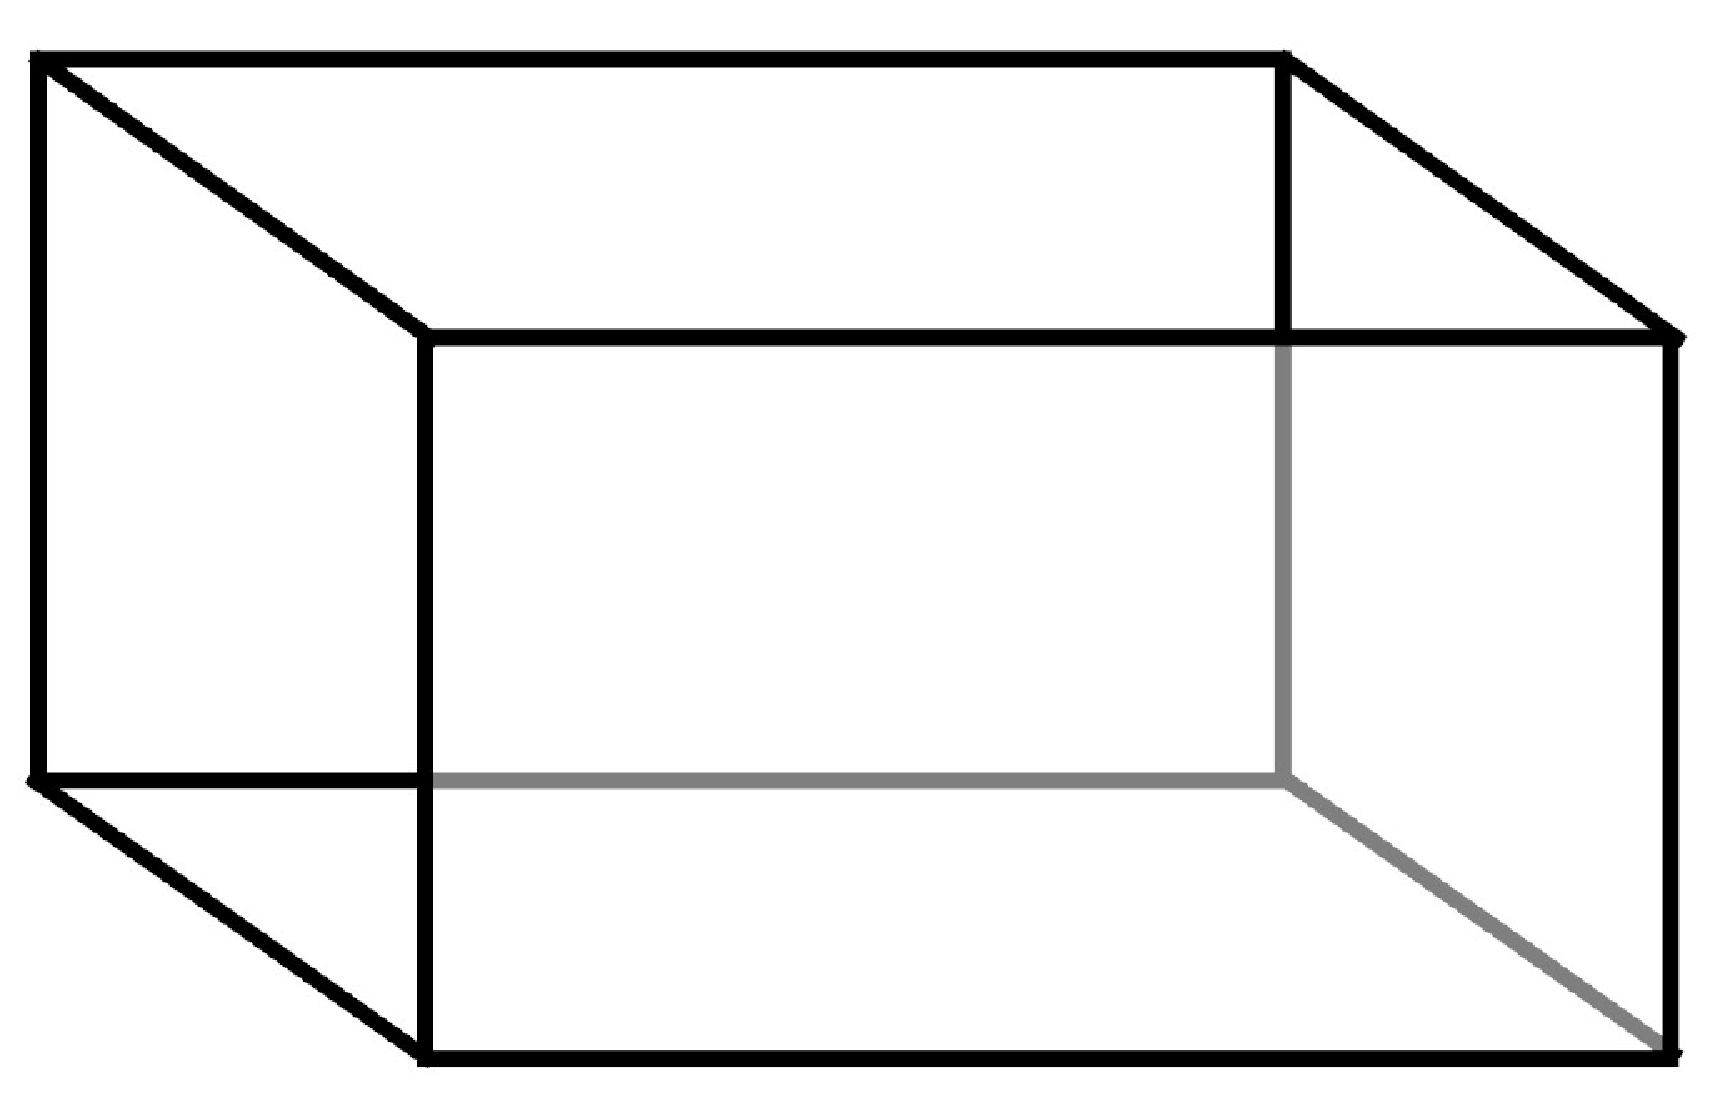
\includegraphics[height=5cm]{ortho.ps}
\caption{The orthorhomic MD cell.}
\end{center}
\end{figure}

\subsubsection*{Parallelepiped periodic boundaries (IMCON=3)}

\begin{figure}[ht]
\begin{center}
\includegraphics[height=5 cm]{triclinic.ps}
\caption{The parallelepiped MD cell.}
\end{center}
\end{figure}

The parallelepiped (e.g. monoclinic or triclinic) cell is generally
used in simulations of crystalline materials, where its shape and
dimension is commensurate with the unit cell of the
crystal. Thus for a unit cell specified by three principal vectors
$\vek{a}$, $\vek{b}$, $\vek{c}$, the MD cell is defined in the \D{}
CONFIG file by the vectors (L$a_{1}$,L$a_{2}$,L$a_{3}$),
(M$b_{1}$,M$b_{2}$,M$b_{3}$), (N$c_{1}$,M$c_{2}$,N$c_{3}$), in which
L,M,N are integers, reflecting the multiplication of the unit cell in
each principal direction. Note that the atomic coordinate origin is
the centre of the MD cell.

The parallelepiped boundary condition can be used with the Ewald summation
method.

\subsubsection*{Truncated octahedral boundaries (IMCON=4)}

\begin{figure}[ht]
\begin{center}
\includegraphics[height=5 cm]{octa.ps}
\caption{The truncated octahedral MD cell.}
\end{center}
\end{figure}

This is one of the more unusual MD cells available in DL\_POLY, but it
has the advantage of being more nearly spherical than most other MD
cells. This means it can accommodate a larger spherical cutoff for a
given number of atoms, which leads to greater efficiency. This can be
very useful when simulating (for example) a large molecule in
solution, where fewer solvent molecules are required for a given
simulation cell width.

The principal axes of the truncated octahedron (see figure) pass
through the centres of the square faces, and the width of the cell,
measured from square face to square face along a principal axis
defines the width D of the cell. From this, the cell vectors required
in the \D{} CONFIG file are simply: (D,0,0), (0,D,0), (0,0,D). These are
also the cell vectors defining the enscribing cube, which posseses
twice the volume of the truncated octahedral cell.  Once again, the
atomic positions are defined with respect to the cell centre.

The truncated octahedron can be used with the Ewald summation method.

\subsubsection*{Rhombic dodecahedral boundaries (IMCON=5)}
This is another unusual MD cell (see figure), but which possesses
similar advantages to the truncated octahedron, but with a slightly
greater efficiency in its use of the cell volume (the ratio is about
74\% to 68\%).

The principal axis in the X-direction of the rhombic dodecahedron
passes through the centre of the cell and the centre of a rhombic
face. The Y-axis does likewise, but is set at 90 degrees to the
X-axis.  The Z-axis completes the orthonormal set and passes through a
vertex where four faces meet. If the width D of the cell is defined as
the perpendicular distance between two opposite faces, the cell
vectors required for the \D{} CONFIG file are: (D,0,0), (0,D,0),
(0,0,$\sqrt{2}$D).These also define the enscribing orthorhombic cell,
which has twice the MD cell volume.  In \D{} the centre of the cell is
also the origin of the atomic coordinates.

The rhombic dodecahedron can be used with the Ewald summation
method.

\begin{figure}[ht]
\begin{center}
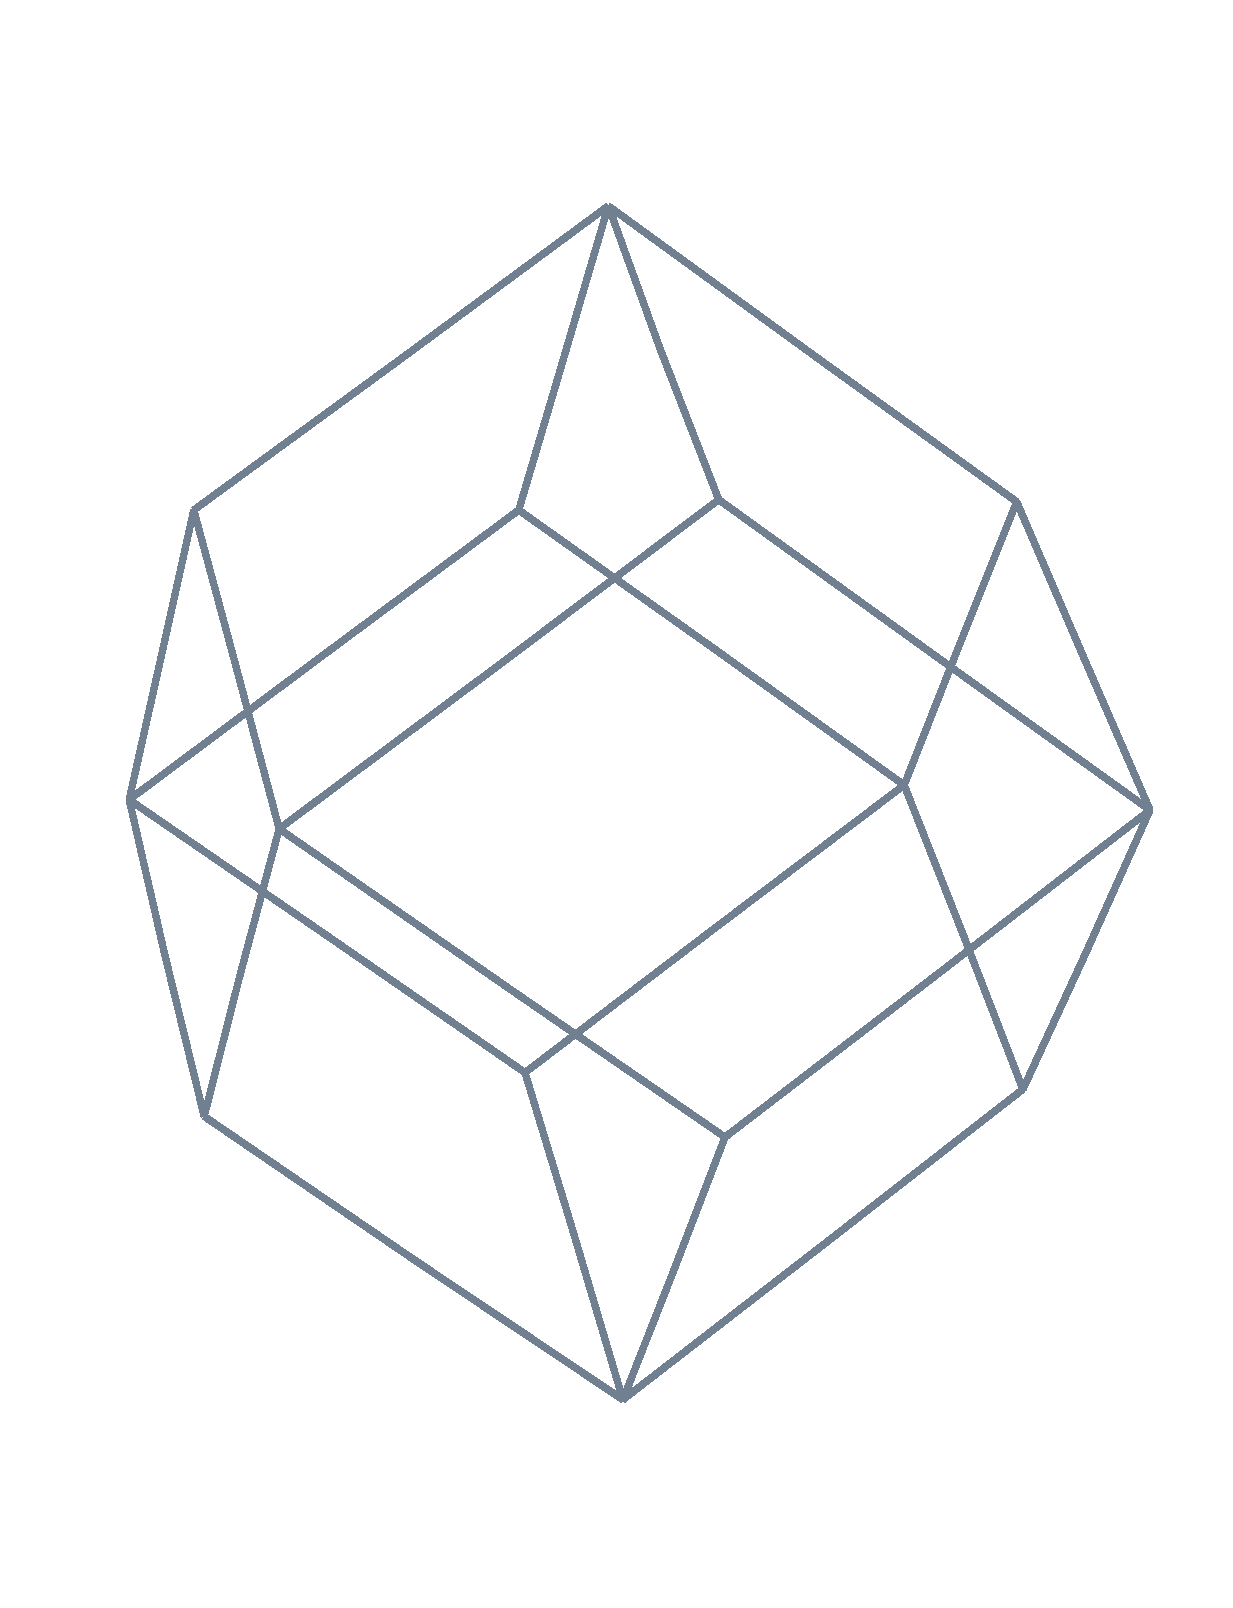
\includegraphics[height=5 cm]{rhombic.ps}
\caption{The rhombic dodecahedral MD cell.}
\end{center}
\end{figure}

\subsubsection*{Slab boundary conditions (IMCON=6)}

Slab boundaries are periodic in the X- and Y-directions, but not in
the Z-direction. They are particularly useful for simulating surfaces.
The periodic cell in the XY plane can be any parallelogram. The origin
of the X,Y atomic coordinates lies on an axis perpendicular to the
centre of the parallelogram. The origin of the Z coordinate is where
the user specifies it, but at or near the surface is recommended.

If the XY parallelogram is defined by vectors $\vek{A}$ and $\vek{B}$,
the vectors required in the CONFIG file are: (A$_{1}$,A$_{2}$,0),
(B$_{1}$,B$_{2}$,0), (0,0,D), where D is any real number (including
zero). If D is nonzero, it will be used by DL\_POLY to help determine
a `working volume' for the system. This is needed to help calculate
RDFs etc. (The working value of D is in fact taken as one of:
3$\times$cutoff; or 2$\times$max~abs(Z coordinate)+cutoff; or the user
specified D, whichever is the larger.)

Note that the standard Ewald sum cannot be used with this boundary
condition. \D{} switches automatically to the Hautman-Klein-Ewald method
instead \cite{hautman-92a}. \index{Ewald!Hautman Klein} 

The surface in a system with charges can also be modelled with \D{} if
periodicity is allowed in the Z-direction. In this case slabs of
ions well-separated by vacuum zones in the Z-direction can be handled
with IMCON=2 or 3.

\subsubsection*{Hexagonal prism boundaries (IMCON=7)}

In this case the Z-axis lies along a line joining the centres of the
hexagonal faces. The Y-axis is perpendicular to this and passes
through the centre of one of the faces. The X-axis completes the
orthonormal set and passes through the centre of an edge that is
parallel to the Z-axis. (Note: It is important to get this convention
right!) The origin of the atomic coordinates is the centre of the
cell. If the length of one of the hexagon edges is D, the cell vectors
required in the CONFIG file are: (3D,0,0), (0,$\sqrt{3}$D,0), (0,0,H),
where H is the prism height (the distance between hexagonal
faces). The orthorhombic cell also defined by these vectors enscribes the
hexagonal prism and possesses twice the volume, but the height
and the centre are the same. 

The Ewald summation method may be used with this periodic boundary condition.

\begin{figure}[ht]
\begin{center}
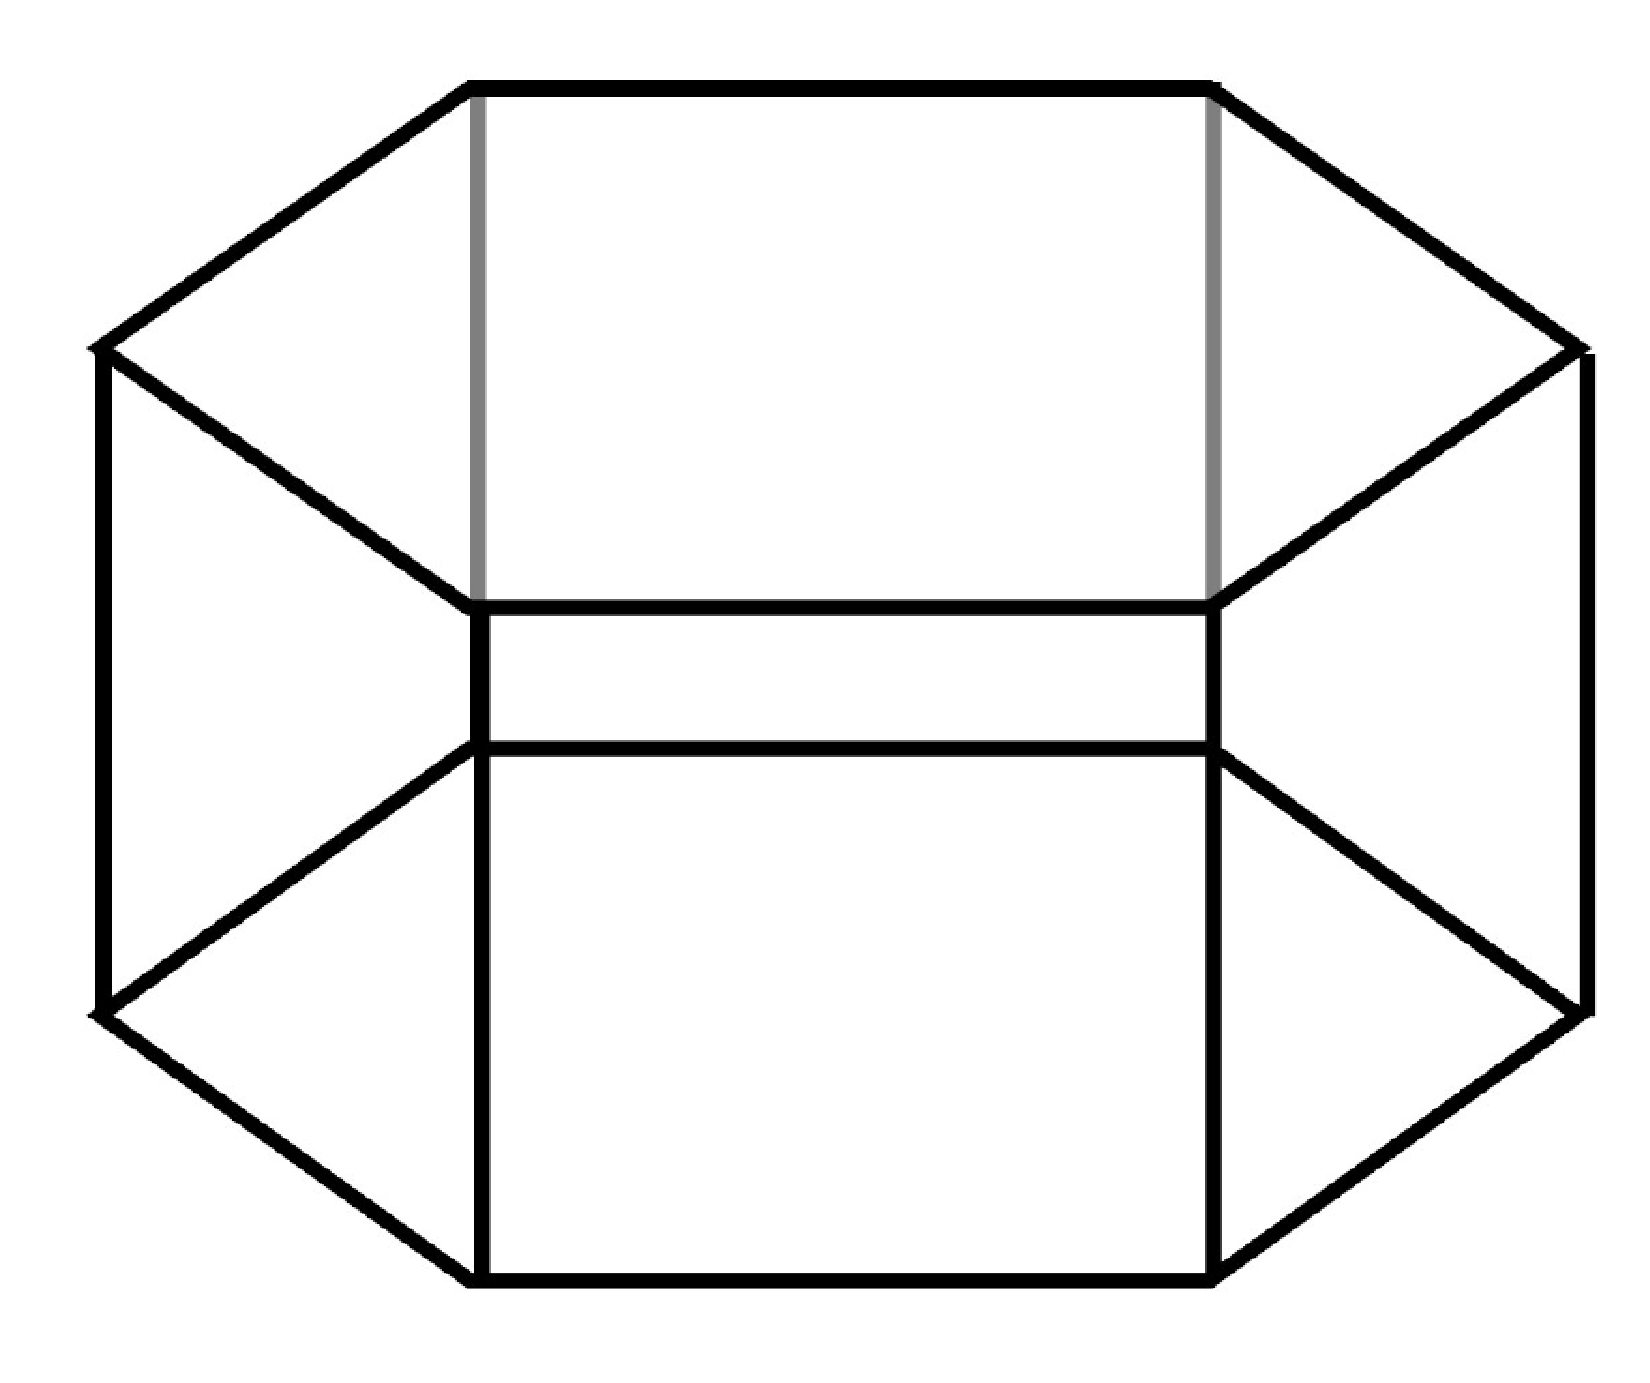
\includegraphics[height=5 cm]{hexa.ps}
\caption{The hexagonal MD cell.}
\end{center}
\end{figure}

This MD cell is particularly suitable for simulating strands or fibres
(i.e. systems with a pronounced anisotropy in the Z-direction), such as
DNA strands in solution, or stretched polymer chains.
